\chapter{Test und Verbesserungen des Detroits}
In diesem Kapitel wird beschrieben, wie überprüft wurde, ob der Aufbau funktioniert. Da Batterie und Fahrzeug lange zwei unabhängige Teilprojekte waren, wurden diese zuerst einzeln komplett getestet, um anschliessend kombiniert erneut getestet zu werden.

Sämtliche Tests erfolgten dabei nach dem Prinzip, immer möglichst kleine Baugruppen einzeln und diese anschliessend in grösseren Baugruppen zu testen.

Die bei den Tests gewonnenen Erkenntnisse konnten nicht komplett während der Projektarbeit umgesetzt werden. Deswegen wird am Ende dieses Kapitels auf gefundene Schwachstellen eingegangen, welche nicht sicherheitsrelevant sind und grössere Umbaumassnahmen erfordern und deswegen nicht durchgeführt wurden. Doch auch ohne diese Umbauten funktioniert der \textsc{Detroit} korrekt und sicher, weswegen diese Massnahmen schon fast als "`Schönheitskorrekturen"' bezeichnet werden können.

\section{Test des Fahrzeugs}
Um das Fahrzeug ohne Batterie testen zu können, muss eine leistungsstarke Gleichspannungsquelle zur Verfügung stehen. Diese arbeitet nach dem Prinzip der Gleichrichtung der Netzspannung, wobei anschliessend noch eine Glättung erfolgen kann. Zu diesem Zweck wurde eine Spannungsquelle der FHNW wieder hergerichtet und mit neuen Steckbuchsen versehen. Diese ist im aktuellen Zustand in Abbildung \ref{fig:Spannungsquelle_blau} zu sehen.

\begin{figure}[h]
	\centering
		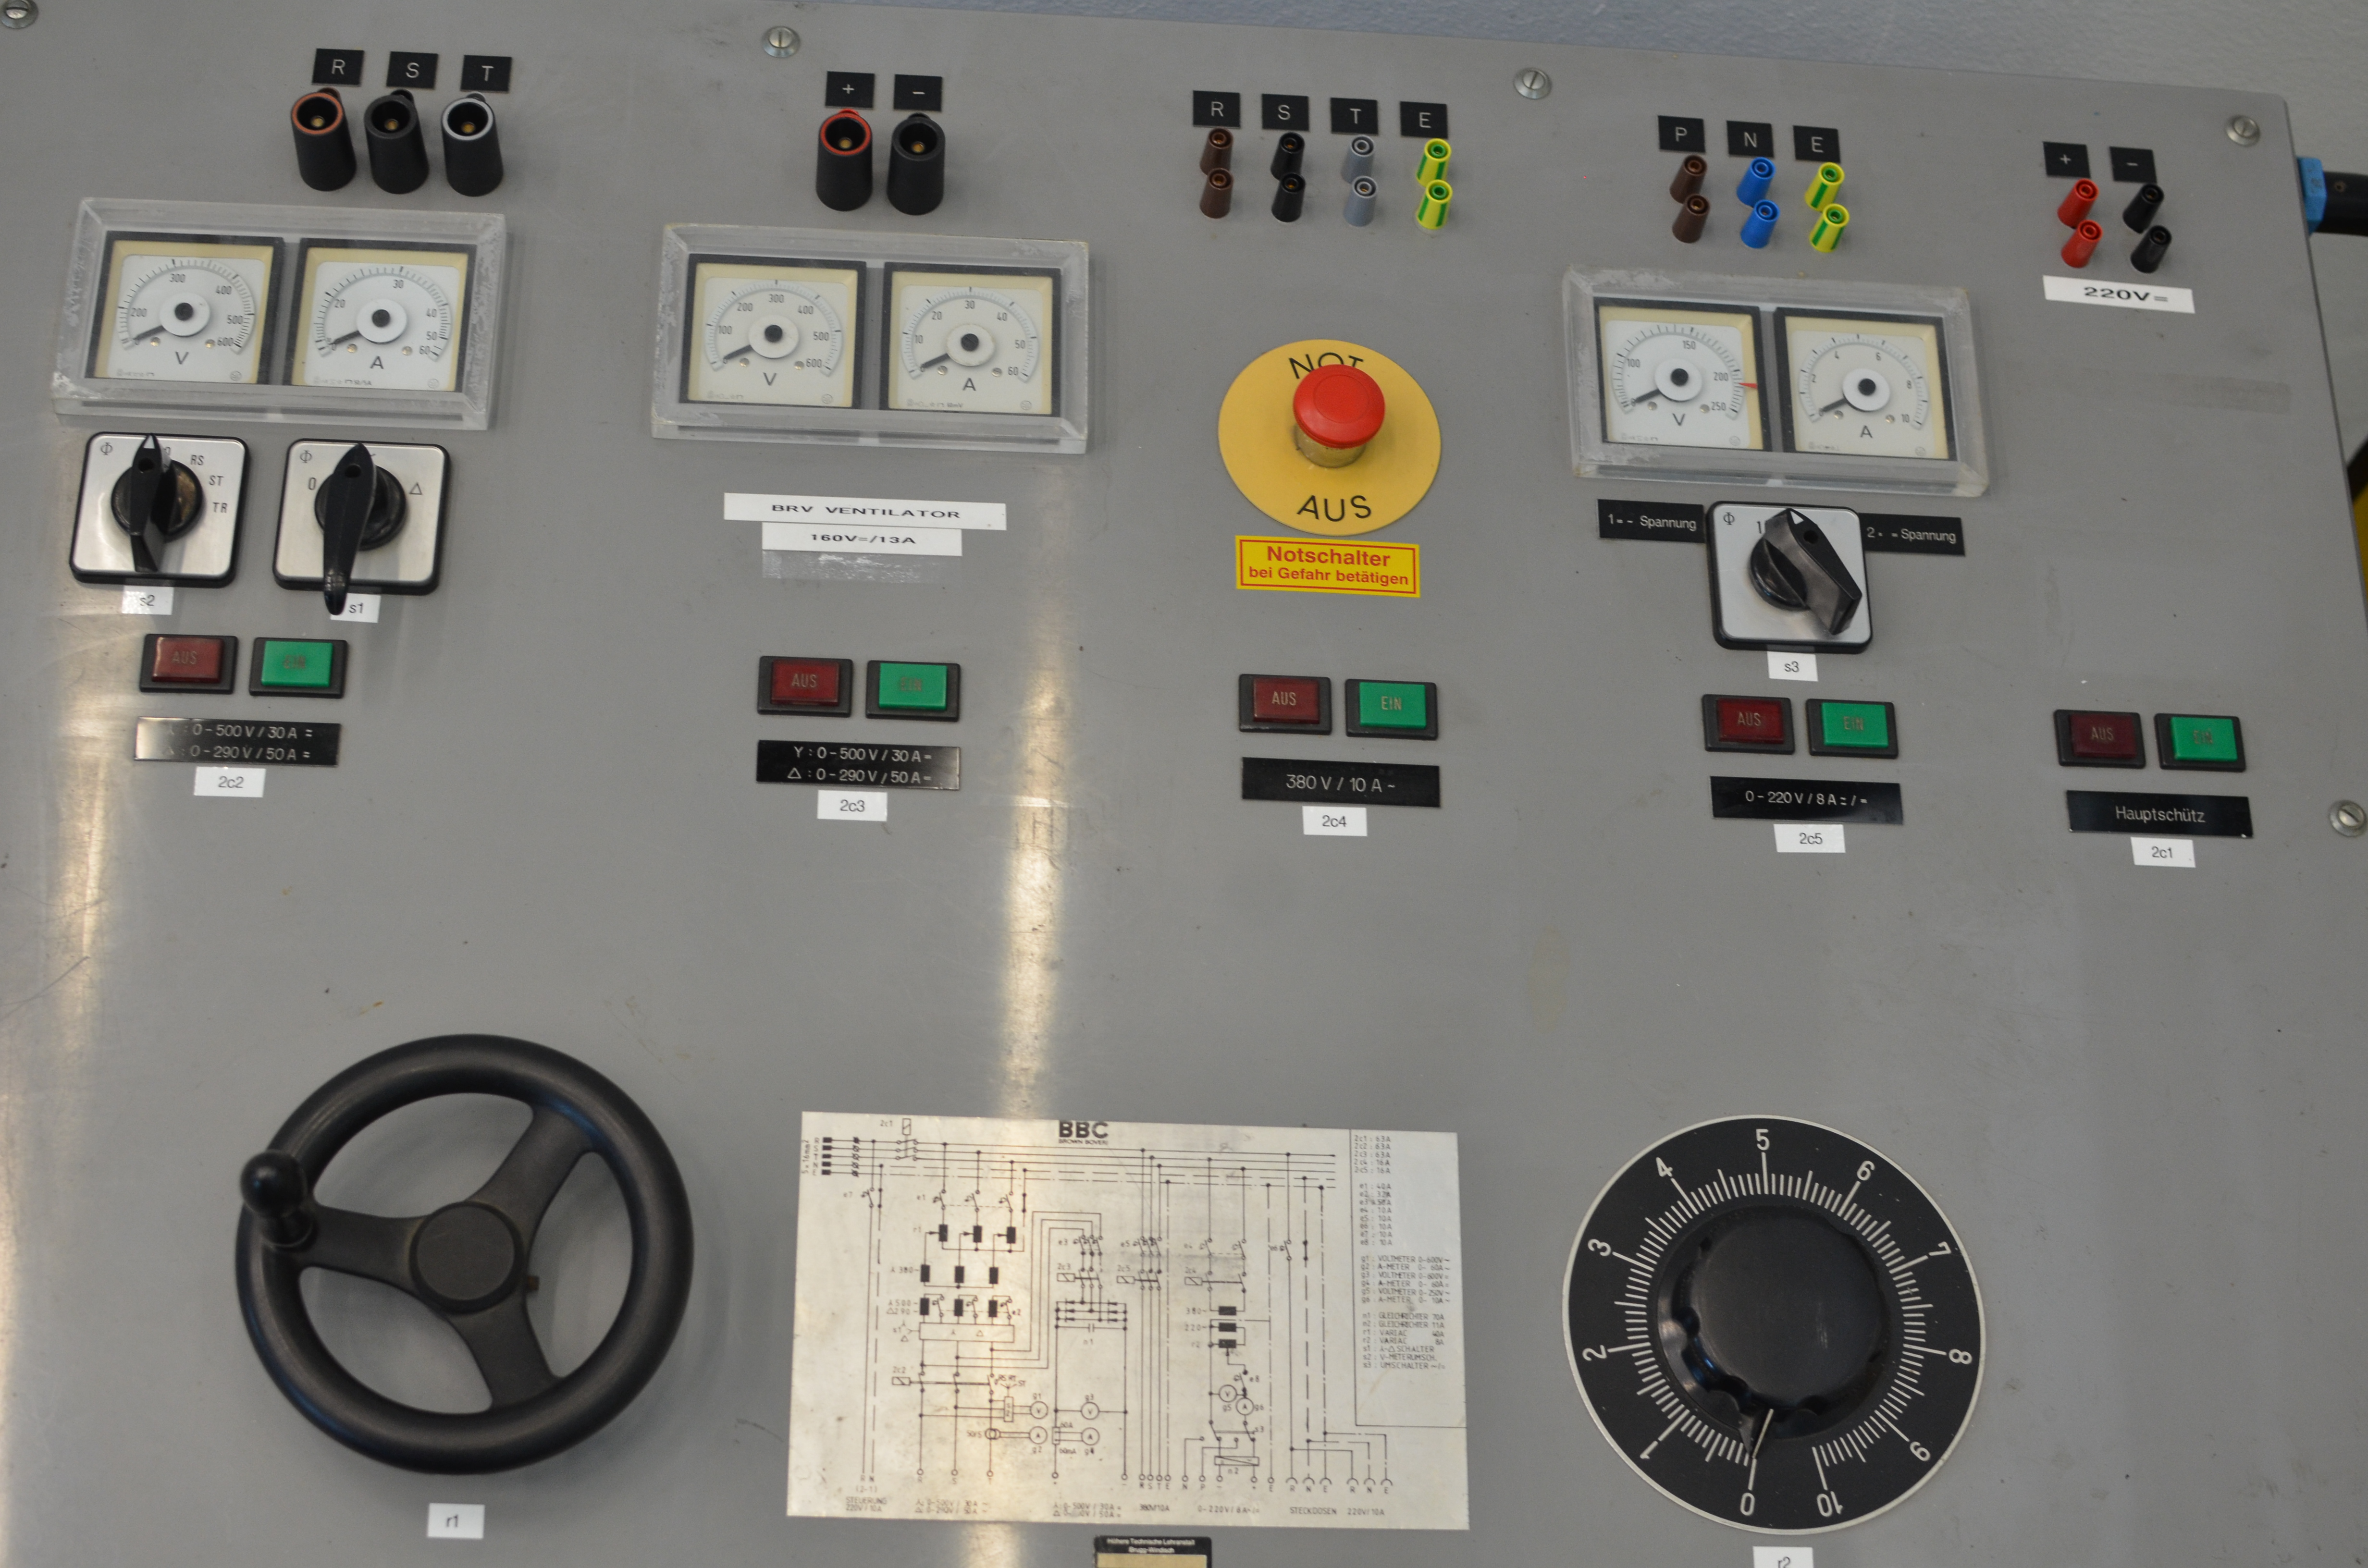
\includegraphics[width=0.80\textwidth]{images/Spannungsquelle.jpg}
	\caption{Die zur Prüfung verwendete Spannungsquelle}
	\label{fig:Spannungsquelle_blau}
\end{figure}

Diese Quelle ist in der Lage, bei Gleichspannung einen maximalen Strom von $70$ A zu liefern, was für Testzwecke ausreichend ist. Weitere Funktionen der Quelle, welche jedoch für das Projekt nicht benötigt wurden, sind eine regelbare Dreiphasen-Wechselspannung, eine regelbare Einphasen-Wechselspannung, eine weitere regelbare Gleichspannung kleiner Leistung sowie $230$ V Steckdosen. Sämtliche Abgänge sind dabei galvanisch getrennt.

Um die unteren Fahrstufen zu überprüfen, wurde die Spannungsquelle an die Anschlüsse der Heckbatterie angeschlossen, da bei diesen Stufen die Batterien parallel geschaltet sind. Da der Motor so nicht in Bewegung gesetzt werden konnte, wurde die Fehlersuche durch Messen einer anliegenden Spannung an folgenden Komponenten durchgeführt: \newpage\begin{itemize}
	\item Anschlüsse der zweiten Batterie
	\item Stufenschalter und Shunt
	\item Bürsten des Motors
	\item Vorwärts-Rückwärts-Schalter
	\item Hauptschalter
\end{itemize}

Das Problem konnte letztlich gefunden und behoben werden. Der originale Hauptschalter ist mechanisch an die Handbremse gekoppelt und sollte so beim Lösen von letzterer auch eingeschaltet werden. Da die Kontakte sehr stark korrodiert waren, reichte die Kraft der Feder nicht mehr, um eine elektrische Verbindung herzustellen. Die Funktion des originalen Hauptschalters konnte nicht wiederhergestellt werden. Stattdessen konnte diese durch einen neuen gasisolierten Schalter sichergestellt werden und der alte Schalter gemäss Kapitel \ref{orig_HS} überbrückt werden.

Weitere Fehler im Antriebsstrang des Fahrzeuges konnten nicht gefunden werden, sodass festgehalten werden kann, dass dieser Bereich des Fahrzeuges bereits zu Beginn des Projektes in einem guten Zustand war.

Für die Tests der höheren Fahrstufen wurde der Pluspol des einen Batteriekabels mit dem Minuspol des anderen Batteriekabels verbunden und die Spannungsquelle mit höherer Spannung an die beiden übrig gebliebenen Kontakte angeschlossen. Auch in dieser Stellung konnten keine Fehler gefunden werden.



\newpage